\chapter{Introduction}

\section{Motivation and related work}



Epidemiology \cite{human_sex}, personal health issues \cite{Madan}, group discovery \cite{5591535}, human mobility \cite{Sun2011929,sevtsuk}, efficient team creation \cite{ECTA, Pentland}, the analysis of academic success \cite{academics}, network theory \cite{networks}, also Fig. \ref{pic:dynamicsf2f}, and psychological research \cite{Rachuri}; all of the above have begun making use of the same notion, one that is difficult to quantify \cite{quant, Wilson}: social connections and social interactions between individuals. And although co-location does not necessarily mean physical social interaction, it is a requirement for it. \cite{Eagle08092009}.

\begin{figure}[h]
	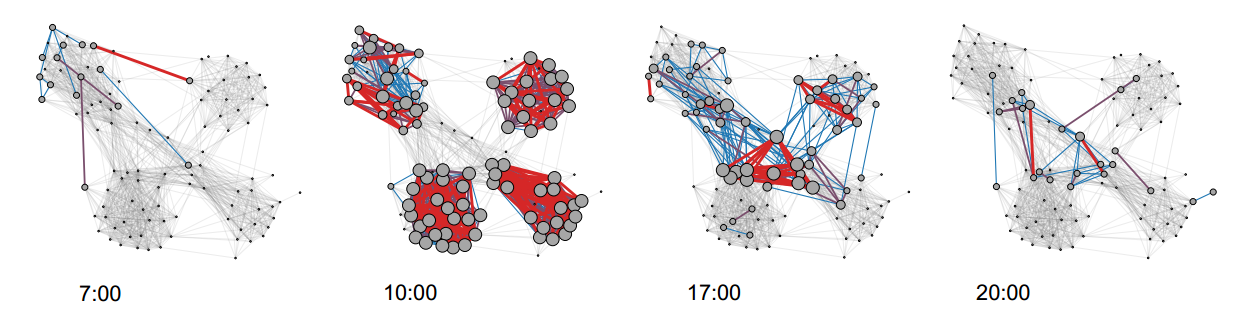
\includegraphics[scale=0.35]{figures/dynamicsf2f.png}
	\caption{Face-to-face interactions over a day for college students. Blue means a low, and red a high frequency of interactions. Image from \protect\cite{Stopczynski}}.
	\label{pic:dynamicsf2f}

\end{figure} 

There are a number of approaches to determining co-location: self-reported data, a more traditional approach, which is prone to cognitive bias, social desirability bias and halo error \cite{Wuchty08092009,gonyea}. A more recent approach involves the use of data provided by modern means of communication, namely mobile phones. This data can come from both the actual phone, in the form of GPS locations or bluetooth readings \cite{Stopczynski}, as well as from the phone company itself in the form of anonymous cell tower records \cite{Onnela01052007, hovel}. This has the advantage of being applicable almost anywhere, because of the high percentage of mobile phone penetration (95.5\% estimated by the International Telecommunication Union in May 2014). 
However, there are approaches that yield better results, but come with financial, environmental or other types of additional cost.

In \cite{catt}, \textit{Barrat and Cattuto} use RFID tags as means to collect data. The tags are embedded into badges, that are worn by the study participants. Radio receivers are installed in the environment that save and pre-process the data sent by the tags. While the face-to-face proximity can be determined with high accuracy (99\%), the cost and effort of creating and distributing the badges, and the limitations imposed by the enclosed area where the receivers are installed make this method hard to use on a large scale.

As a data source, in \cite{audiovideo}, \textit{Wyatt et. al} used audio-video recordings. The study participants wore an over-the-shoulder bag which contained a PDA and a multi-sensor board, which received information from a multitude of sensors located on the user, including a microphone.

\textit{Sociometric} badges were used as means of collecting data by \textit{Olguin et al.} in \cite{onbody}. The badges are the size of a mobile phone, and record a high amount of information from a variety of sensors: common human daily activities, speech features, indoor user localization and face-to-face interaction time, in addition to Bluetooth detection and communication with receivers in the environment.

In \cite{wifi}, \textit{ Kjærgaard and Nurmi} use the WiFi capabilities on smartphones. While being usable both indoors and outdoors, the authors present a number of challenges that have to be overcame before this method can be used for social discovery on a larger scale.   
 
\section{Objective}

Given a bluetooth RSSI between two phones, the purpose of this paper is to indicate a method which reliably and accurately determines the existence of pairwise co-location between the people carrying the two phones.
 
The inference of co-location is achieved by applying and analysing multiple machine learning algorithms on a data set consisting of two main parts:
\begin{itemize}
  \item Data automatically recorded by the SensibleDTU data collector app \cite{Stopczynski}
  \item Ground truth data obtained by the test subjects by interacting with the FriendFinder app
\end{itemize}

For each machine learning algorithm the parameter configuration which yields the best results will be chosen, followed by a comparison between the best configurations for each algorithm.      

\section{Scope and limitations}

The paper analyses the data obtained from three test subjects. Each subject has been given the same phone model, Samsung Galaxy Nexus. The app built for the phones, FriendFinder, has a purely functional purpose. As such, little to no consideration has been given to the style, theme or design of the app. Fig \ref{pic:ff_prtscr} shows the app, and while fit for purpose, it is not very aesthetic.

While considerable testing has been done with regards to the algorithm parameters, the machine learning algorithms used are by no means exhaustive. There are three main algorithms: Naive Bayes, neural networks, and logistic regression.

When analysing data, we only look at the bluetooth RSSI value, and data derived directly while measuring it. For example, given that measurements are taken every five minutes, we at some point look at the number of uninterrupted measurements, or at the measurements taken before and after (if possible) a specific measurement. GPS traces, phone records, infrared sensors, or facebook/email information are not taken into consideration.

\section{Thesis Outline}

The thesis begins with this introduction, which gives an overview of the general theme of the project. The objectives, scope and limitations and thesis outline are all self-defining. 

The paper continues with a section which describes the data acquisition process and the methodology used to obtain the data from the SensibleDTU database. The section also describes the FriendFinder app, as well as its implementation.

Next, the machine learning algorithms are presented. For each algorithm a theoretical overview is given. The implementation details are discussed, followed by the results obtained by applying it to the data. At the end of this chapter, we do a comparative analysis between the algorithms, followed by the last section, the conclusions, where we will give the final results and recommendations.
